\section{Flip-Consistent Training}
\label{sec:method}

FCT is a training loss. It replaces the supervised loss of a segmentation network with three parts:
the supervised loss on three orientation views of each image, a consistency term that draws the
predictions of the views together, and label-aware weights that decide, pixel by pixel, how much
each view may move toward another (Fig.~\ref{fig:overview}). The network and its inference are
unchanged. This section describes the three parts and the full loss, and then relates FCT to other
losses.

\begin{figure*}[t]
\centering
% Overview of FCT (Section IV). Needs \usepackage{tikz} and
% \usetikzlibrary{arrows.meta,positioning,calc,fit,backgrounds}.
% Thumbnails: figures/ov/*.png (a Kvasir-SEG training image, its two flips and its label).
\definecolor{flipc}{HTML}{2A78D6}
\definecolor{upc}{HTML}{EB6834}
\begin{tikzpicture}[
  font=\footnotesize, >={Stealth[length=4.2pt,width=3.8pt]},
  img/.style={inner sep=0pt, draw=black!35, line width=0.3pt},
  net/.style={draw=black!70, line width=0.5pt, fill=black!4, rounded corners=1.5pt,
              minimum width=9mm, minimum height=7mm, align=center},
  map/.style={draw=black!70, line width=0.5pt, fill=white, minimum width=8mm, minimum height=7mm},
  sup/.style={draw=black!60, line width=0.4pt, fill=black!4, rounded corners=1.5pt,
              minimum height=5.5mm, inner xsep=2.5pt, align=center},
  flow/.style={->, line width=0.5pt, black!75},
  pull/.style={->, line width=1.2pt},
  lab/.style={font=\scriptsize, black!85, align=center},
]
  \def\th{10.5mm}
  % ---- inputs: the image and its two flips -------------------------------------
  \node[img] (xh) at (0, 1.45)  {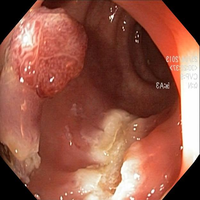
\includegraphics[width=\th]{figures/ov/xh.png}};
  \node[img] (x)  at (0, 0)     {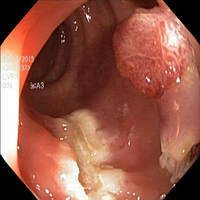
\includegraphics[width=\th]{figures/ov/x.png}};
  \node[img] (xv) at (0, -1.45) {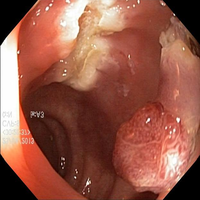
\includegraphics[width=\th]{figures/ov/xv.png}};
  \node[lab, left=1.2mm of xh] {$T_h x$};
  \node[lab, left=1.2mm of x]  {$x$};
  \node[lab, left=1.2mm of xv] {$T_v x$};
  % ---- one network, three passes ------------------------------------------------
  \node[net] (fh) at (1.6, 1.45)  {$f$};
  \node[net] (fo) at (1.6, 0)     {$f$};
  \node[net] (fv) at (1.6, -1.45) {$f$};
  \draw[flow] (xh) -- (fh); \draw[flow] (x) -- (fo); \draw[flow] (xv) -- (fv);
  \begin{scope}[on background layer]
    \node[draw=black!35, dashed, line width=0.4pt, rounded corners=2pt, fit=(fh)(fv), inner sep=2.2mm] (shared) {};
  \end{scope}
  \node[lab, below=0.6mm of shared] {shared weights,\\ same depth mask};
  % ---- logits in the upright frame -----------------------------------------------
  \node[map] (zh) at (3.45, 1.45)  {$z^{h}$};
  \node[map] (zo) at (3.45, 0)     {$z^{o}$};
  \node[map] (zv) at (3.45, -1.45) {$z^{v}$};
  \draw[flow] (fh) -- node[lab, above, pos=0.62] {$T_h^{-1}$} (zh);
  \draw[flow] (fo) -- (zo);
  \draw[flow] (fv) -- node[lab, above, pos=0.62] {$T_v^{-1}$} (zv);
  % ---- (1) the three supervised views ---------------------------------------------
  \node[sup] (sh) at (5.2, 1.45)  {$\tfrac13\mathcal{L}_{\mathrm{host}}$};
  \node[sup] (so) at (5.2, 0)     {$\tfrac13\mathcal{L}_{\mathrm{host}}$};
  \node[sup] (sv) at (5.2, -1.45) {$\tfrac13\mathcal{L}_{\mathrm{host}}$};
  \draw[flow] (zh) -- (sh); \draw[flow] (zo) -- (so); \draw[flow] (zv) -- (sv);
  \node[img] (y) at (6.85, 0) {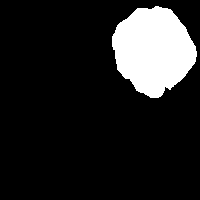
\includegraphics[width=\th]{figures/ov/y.png}};
  \node[lab, below=0.6mm of y] {label $y$};
  \draw[flow, black!45] (y.north west) -- (sh.east);
  \draw[flow, black!45] (y.west) -- (so.east);
  \draw[flow, black!45] (y.south west) -- (sv.east);
  \node[lab, above=1.4mm of sh, xshift=4mm] {(1) three supervised views};
  % ---- (2) the consistency term between the views' probabilities -----------------
  \node[map] (po) at (8.75, 0)     {$p^{o}$};
  \node[map] (ph) at (10.95, 1.15) {$p^{h}$};
  \node[map] (pv) at (10.95, -1.15) {$p^{v}$};
  \draw[pull, flipc] (po.north) to[bend left=28] node[lab, above left, pos=0.45, xshift=1mm] {$C_h$, weight $w_h$} (ph.west);
  \draw[pull, upc]   (ph.south) to[bend left=28] (po.east);
  \draw[pull, flipc] (po.south) to[bend right=28] node[lab, below left, pos=0.45, xshift=1mm] {$C_v$, weight $w_v$} (pv.west);
  \draw[pull, upc]   (pv.north) to[bend right=28] (po.east);
  \node[lab] at (9.95, 0.47) {$U$, gate $g$};
  \node[lab] at (9.85, 2.25) {(2) label-aware consistency, $p=\sigma(z)$};
  \node[lab, anchor=west] at (11.55, 0.35) {\textcolor{flipc}{\rule[0.5ex]{3mm}{1.2pt}} flipped views:};
  \node[lab, anchor=west] at (11.55, 0.0) {lag or margin};
  \node[lab, anchor=west] at (11.55, -0.45) {\textcolor{upc}{\rule[0.5ex]{3mm}{1.2pt}} upright view:};
  \node[lab, anchor=west] at (11.55, -0.8) {best flip, gated};
  \node[lab] at (9.85, -2.2) {arrow: detached target $\to$ view it moves};
\end{tikzpicture}

\caption{Overview of the FCT loss. (1)~An image and its horizontal and vertical flips pass through one
network; the flipped outputs are flipped back, and each view is supervised with the host network's own
loss, weighted $\frac13$. (2)~A consistency term draws the predictions of the views together, each
toward a detached target: the flipped views toward the upright view, with the lag-or-margin weight of
Eq.~\eqref{eq:weight}, and the upright view toward the flipped view closest to the label, wherever that
view is more accurate. At test time, only the upright view is used.}
\label{fig:overview}
\end{figure*}

\subsection{Multi-View Supervision}
\label{sec:views}

Each image is passed through the network upright and flipped horizontally and vertically, and the
flipped outputs are flipped back to the upright frame as in Eq.~\eqref{eq:views}. Every view is
supervised with the host network's own loss:
\begin{equation}
\mathcal{L}_{\mathrm{sup}}=\frac13\sum_{k\in\{o,h,v\}}\mathcal{L}_{\mathrm{host}}\big(Z^{k},y\big),
\label{eq:sup}
\end{equation}
where $Z^{k}$ denotes all output maps of view $k$ in the upright frame and $\mathcal{L}_{\mathrm{host}}$
the supervised loss of the host network, unchanged; the prediction logit $z^{k}$ is formed from $Z^{k}$
as the host forms it at test time. The factor $\frac13$ keeps the supervised loss at the scale of
single-view training. On its own, Eq.~\eqref{eq:sup} is a deterministic form of flip augmentation:
each view is tied to the label, but no view is tied to another.

\subsection{Cross-View Consistency}
\label{sec:flippull}

The consistency term ties the views to each other. It draws each flipped view $k$ toward the detached
upright prediction,
\begin{equation}
\mathcal{C}_k=\frac{1}{HW}\sum_{i} w^{k}_i\,\ell\big(z^{k}_i;p^{o}_i\big),
\label{eq:flippull}
\end{equation}
with the weights $w^{k}_i$ of Section~\ref{sec:weights}, and it draws the upright view toward the flipped
view closest to the label, wherever that view is more accurate:
\begin{equation}
\mathcal{U}=\frac{1}{HW}\sum_{i} g_i\,\ell\big(z^{o}_i;p^{\ast}_i\big),\qquad g_i=\mathbf{1}\big[e^{\ast}_i<e^{o}_i\big],
\label{eq:uppull}
\end{equation}
where $p^{\ast}_i$ denotes the detached probability of the flipped view with the smaller error at
pixel $i$, and $e^{\ast}_i$ its error. Together, the two directions let the more accurate side move the
other: where the upright view is more accurate, the flipped views move toward it, and where a flipped
view is more accurate, the upright view, which is the one used at test time, moves toward it. By
Corollary~\ref{cor:lag}, every movement that the gate $g$ allows in Eq.~\eqref{eq:uppull} is toward the
label.

\subsection{Label-Aware Weights}
\label{sec:weights}

The weights decide how much each flipped view moves toward the upright view. Following
Corollary~\ref{cor:lag}, the term keeps its full weight where the flipped view lags behind the upright
view, and it is weakened where the flipped view leads:
\begin{equation}
w^{k}_i=\begin{cases}1, & e^{k}_i\geq e^{o}_i,\\ \max\big(0,\,1-a\,e^{o}_i\big), & e^{k}_i<e^{o}_i,\end{cases}
\label{eq:weight}
\end{equation}
where $e^{k}_i$ and $e^{o}_i$ denote the errors of the flipped and the upright view at pixel $i$, computed
without gradient, and $a>0$ is a constant.

The constant $a$ follows from the decision threshold. On a leading pixel, the term moves the flipped
view away from the label (Corollary~\ref{cor:lag}), and Eq.~\eqref{eq:weight} keeps it in proportion to
the margin $1-a\,e^{o}$. We ask two things of this margin. First, a movement toward a wrong target must
vanish, $w=0$ whenever $e^{o}>\frac12$, which requires $a\geq2$. Second, a movement toward a correct
target must survive however small its margin, $w>0$ whenever $e^{o}<\frac12$, which requires
$a\leq2$. Hence $a=2$, and on a leading pixel with a correct target, $w=1-2e^{o}=|2p^{o}-1|$ is twice
the target's distance from the threshold, that is, its margin rescaled to $[0,1]$. The constant is thus
set by the threshold rather than tuned, and Section~\ref{sec:ablation} shows that the results are
insensitive to it.

With $a=2$, the term on a leading pixel is weak. Its strength $w\,(e^{o}-e^{k})$ is at most
$(1-2e^{o})\,e^{o}\leq\frac18$, against up to one for a supervised step (Fig.~\ref{fig:pull}(c)), and it
vanishes when the flipped view reaches the upright prediction, on the correct side of the threshold. It
thus keeps the two views consistent where both are right, as flip equivariance asks, without reversing a
decision by itself.

\subsection{Full Loss and Training}
\label{sec:objective}

The FCT loss adds the consistency term to the multi-view supervision:
\begin{equation}
\mathcal{L}_{\mathrm{FCT}}=\mathcal{L}_{\mathrm{sup}}+\frac{\lambda}{2}\big(\mathcal{C}_h+\mathcal{C}_v\big)+\frac{\lambda}{2}\,\mathcal{U},
\label{eq:objective}
\end{equation}
where $\lambda\geq0$ weighs consistency against supervision. The two flipped views share $\lambda$, and
the upright view's term receives the weight of one flipped view's. The weight is ramped up linearly at
the start of training,
\begin{equation}
\lambda_t=\lambda\,\min\big(1,\,t/t_0\big),
\label{eq:ramp}
\end{equation}
where $t$ counts the training batches and $t_0$ is the length of the ramp; we use $\lambda=0.5$ and
$t_0=300$.

Three implementation choices keep the views comparable and the memory low. First, the three views of
an image share one stochastic-depth mask~\cite{huang2016stochastic}, so that their differences reflect
the flip rather than the random depth. Second, when a host trains at several input scales, FCT is
applied at every scale. Third, the probabilities $p^{h}$ and $p^{v}$ of Eq.~\eqref{eq:uppull} come from
passes without gradient that leave the running statistics of batch normalization unchanged. In our
current implementation, these passes run before the upright pass and the graph of each view is
released after its backward pass, so only one view's computation graph is held in memory at a time;
the runs reported in Section~\ref{sec:experiments} computed them after the upright pass, which gives
the same loss at a higher peak memory. For each image and input scale, FCT thus runs five forward
passes, three of them with gradients. At test time, the network is applied to the upright image only,
exactly as without FCT, so FCT changes neither the architecture nor its inference cost.

\subsection{Relation to Other Losses}
\label{sec:relation}

By Eq.~\eqref{eq:combined}, FCT is a supervised loss with adaptive pixel weights: on a flipped view,
the supervised weight $\frac13$ is raised where the view lags behind the upright view and slightly
lowered where it leads. This places FCT among losses that reweight pixels. Focal
loss~\cite{lin2017focal} and online hard example mining~\cite{shrivastava2016ohem} weight a pixel by its
own error, and the structure loss of PraNet-style networks~\cite{wei2020f3net} by its distance to a
boundary; FCT weights it by how its error compares with that of another view of the same pixel.

The weights of Eq.~\eqref{eq:weight} also contain the usual consistency rules as special cases or near
neighbours, which Section~\ref{sec:ablation} compares. With $w=1$ everywhere, $\mathcal{C}_k$ is the
unweighted transformation consistency of semi-supervised
segmentation~\cite{bortsova2019consistency,li2021tcsm}, applied here to labeled images; by
Eq.~\eqref{eq:weights}, it mixes positive and negative pixel weights. Confidence
thresholding~\cite{sohn2020fixmatch} keeps the terms whose target is confident, which includes
confidently wrong targets, the case that Corollary~\ref{cor:lag} rules out. Finally, a rule can use the
label to judge the target alone, for example by weighting each pixel by whether and how confidently the
upright view is correct. Such a rule ignores the error of the view being moved, so it cannot tell the
lagging pixels, where the term helps, from the leading ones, where it hurts. Of these rules, only FCT
compares the two errors, as Corollary~\ref{cor:lag} requires.
